\chapter{Educação a Distância e Educação Corporativa}


Por ser inerentemente dependente dos meios de comunicação disponíveis, a educação a distância, modalidade do processo de ensino e aprendizado em que professores e alunos estão separados espacial e/ou temporalmente, teve sua expansão favorecida pela relevância da Internet no mercado moderno. (Moore e Kearsley, 1996 \cite{Moore_Kearsley_1996} apud Albertim e Brauer, 2012 \cite{Albertin_Brauer_2012}) Sua principal característica, a ausência da necessidade de um espaço físico compartilhado, permite seu uso para atender públicos diversos, de difícil acesso, ou em situações em que a educação presencial se tornaria proibitivamente custosa, tornando-a indispensável para os objetivos de educação inclusiva e democratização da educação em escala nacional (Abbad, 2007 \cite{Abbad_2007}). Armengol(1987 \cite{Armengol_1987}, apud Nunes 1994 \cite{Nunes_1994}) apresenta as seguintes características da educação a distância:

\begin{itemize}
     
 \item População estudantil relativamente dispersa,
 \item População estudantil predominantemente adulta,
 \item Cursos que pretendem ser autoinstrucionais,
 \item Cursos pré-produzidos,
 \item Comunicações massivas,
 \item Comunicações organizadas em duas direções,
 \item Estudo individualizado,
 \item Forma mediadora de conversação guiada,
 \item Tipo industrializado de ensino aprendizagem,
 \item Crescente utilização da "Nova Tecnologia Informativa" (Computação),
 \item Tendencia a adotar estruturas curriculares flexíveis,
 \item Custos decrescentes por estudante.
 
\end{itemize}
 
 
  Suas implementações, a través dos diversos meios de comunicação, permitem características distintas para adequar-se a realidades distintas. Em particular, a educação a distância assíncrona, seja ela implementada de maneira informatizada ou impressa, permite ao aluno grande flexibilidade na organização do seu tempo de estudo, adequando-a as realidades da educação de adultos, facilitando e democratizando o acesso á educação continuada. (Abbad, 2007 \cite{Abbad_2007}) Segundo este autor, após um crescimento acelerado na década de 90, "O momento atual é o de consolidação das novas práticas educacionais à distância." Porém, ele indica um aumento de 36.0\% no número de instituições de ensino autorizadas a oferecer cursos a distância entre 2004 e 2006, assim como um aumento da média de horas anuais destinadas ao treinamento em empresas Brasileiras de 39 para 47. A caráter comparativo, o autor indica que este valor era superior ao encontrado na Europa (36 h/ano), na Austrália (34 h/ano), na América Latina (31 h/ano) e nos Estados Unidos (30 h/ano). Este crescimento se da em parte devido ao conceito de aprendizagem ao longo de toda a vida, consequência da realidade profissional do mercado de trabalho moderno altamente competitivo e em constante estado de evolução tecnológica, levando a necessidade de capacitação e reciclagem contínuas por parte dos profissionais. Segundo Delors(2005 \cite{Delors_2005}), perante esta realidade, quatro conjuntos de competências tornam-se centrais a formação do profissional moderno:\\
  
  "O aprender a conhecer", referindo-se a necessidade de aprender não ferramentas ou conteúdos específicos, mas linguagens e metodologias para a aquisição e geração de conhecimento\\\
  "O aprender a fazer", referindo-se a atitudes e habilidades que empoderam o indivíduo a enfrentar situações desconhecidas ou desafiadoras,\\
  "O aprender a viver junto", relacionado as capacidades sociais necessárias para o trabalho em equipes multidisciplinares, \\
  "O aprender a ser", referindo-se ao desenvolvimento integro do ser humano.\\
  
  Segundo Abbad (2007 \cite{Abbad_2007}), a automação das atividades mais simples leva a uma tendência mundial de aumento de complexidade dos trabalhos humanos, em diferentes contextos, além de diminuir a demanda por trabalho operacional, gerando desemprego. 
  Para manter a competitividade em mercados globalizados, muitos países tem recorrido ao conceito de universidades abertas, aproveitando as vantagens da educação a distância para promover oportunidades de estudo em nível superior a parcelas da população com poucas oportunidades de acesso ao estudo convencional. Frente a esta grande demanda por cursos de Educação a Distância, o autor apresenta algumas das dificuldades comuns em cursos por aprendizado a distância, principalmente as altas taxas de evasão, e a importância e dificuldade de desenvolver cursos adequados para o público alvo.
  Ele  apresenta  as característica comuns do mesmo, assim como os desafios gerados por elas e as vantagens do ensino a distância em relação ao ensino tradicional, apresentadas a seguir.
  
\begin{figure}
            \begin{center}
                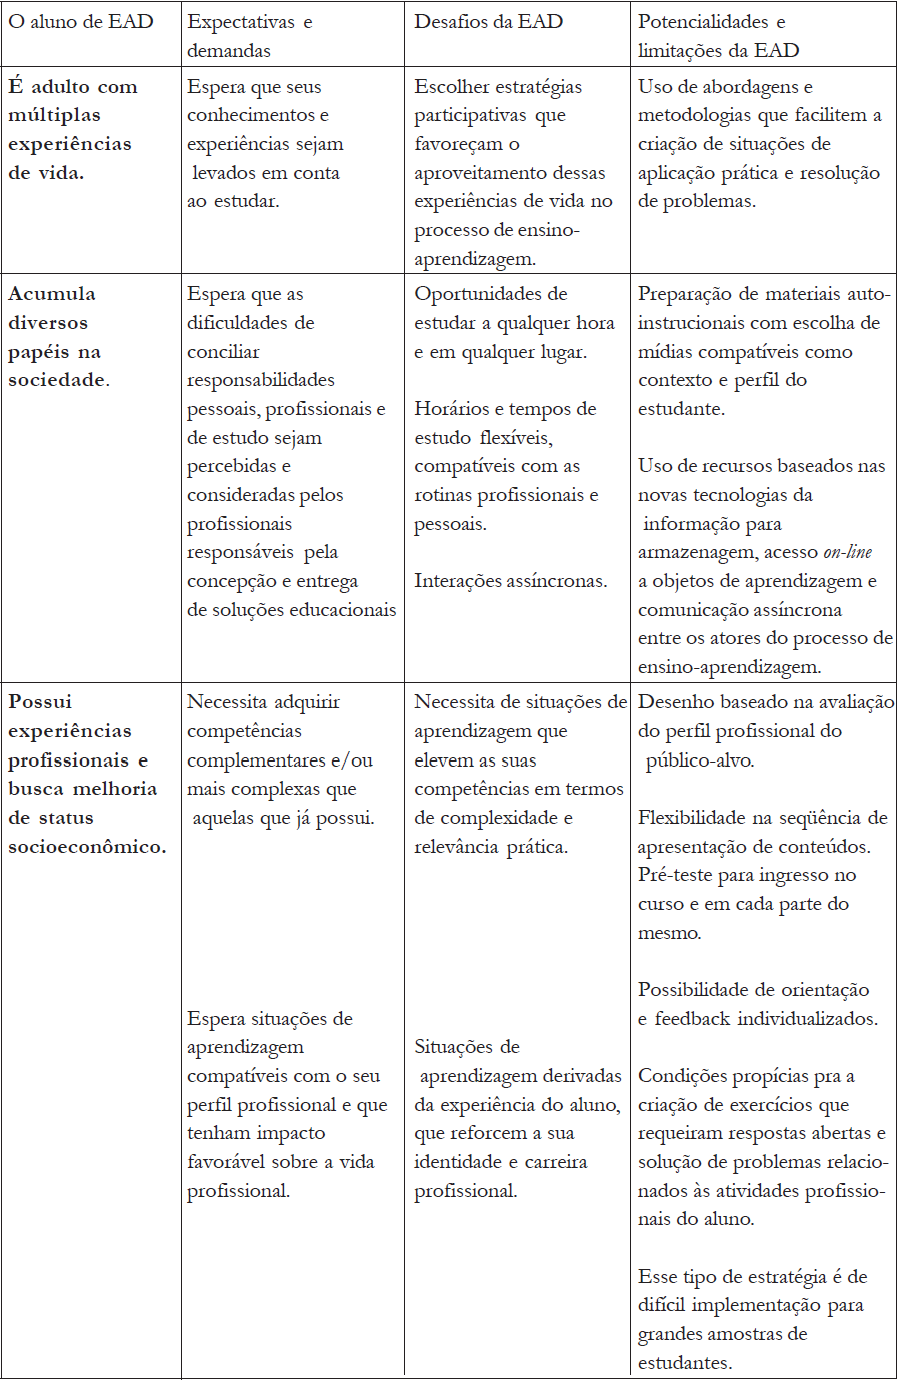
\includegraphics[width=0.9\textwidth]{Tabela_EAD_1_Abbad_2007.png}
            \end{center}
            \caption{A Clientela de EAD (Abbad 2007\cite{Abbad_2007})}
            \label{fig:Clientella_EAD_1}
\end{figure}

  

\begin{figure}
            \begin{center}
                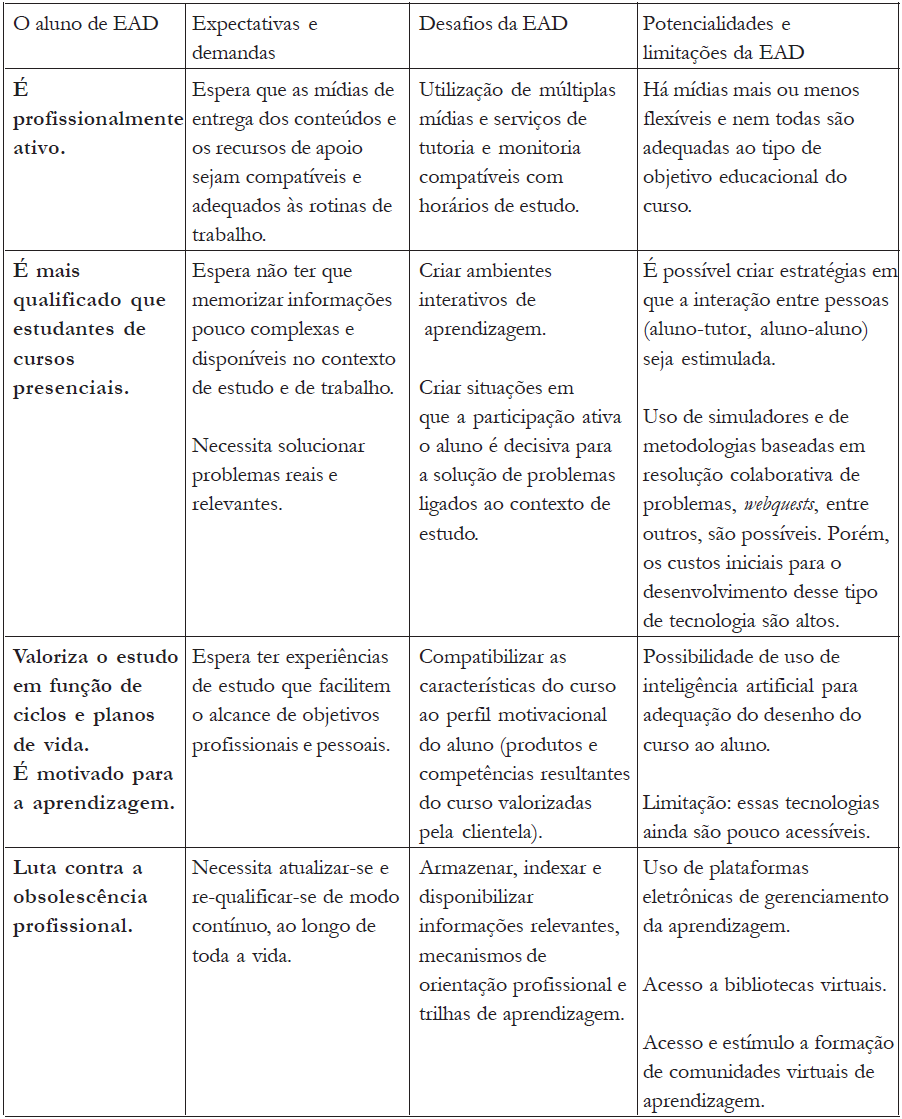
\includegraphics[width=0.9\textwidth]{Tabela_EAD_2_Abbad_2007.png}
            \end{center}
            \caption{A Clientela de EAD (continuação) (Abbad 2007\cite{Abbad_2007})}
            \label{fig:Clientella_EAD_1}
\end{figure}

Além das iniciativas públicas, voltadas a democratização do acesso a educação e a competitividade mercadológica a nível nacional, a realidade atual do mercado globalizado, intensamente dependente das tecnologias da informação e com alta velocidade de evolução, não deixa dúvida sobre a importância da educação continuada para as organizações privadas. Seja para permitir maior produtividade, seja como atrativo para evitar a evasão de mão de obra qualificada, muitas empresas reconheceram a necessidade de providenciar a seus funcionários oportunidades de estudo para manter sua competitividade no mercado globalizado atual. Em vista da complexidade do processo educativo, e de seu alto custo, a eficácia e a eficiência tornam-se preocupações centrais. A partir da década de 50, nos Estados Unidos, empresas de grande porte começaram a implementar Universidades Corporativas de maneira a centralizar seus processos de treinamento (Freitas-Dias e Albuquerque, 2014\cite{Freitas_Albuquerque_2014}, permitindo maior controle sobre o processo educativo. Jeanne Meister (1999 \cite{Meister_1999}, ) define Universidade corporativa como "um guarda-chuva estratégico para desenvolver e educar  funcionários, clientes, fornecedores e comunidade, a fim de cumprir as estratégias empresariais da organização". Vergara (2000 \cite{Vergara_2000}, apud Freitas-Dias e Albuquerque, 2014 \cite{Freitas_Albuquerque_2014}) destaca a importância das universidades corporativas na criação e manutenção da base de conhecimento da empresa, e salienta o ganho em eficiência devido a criação de um código comum de referência para a empresa, seus colaboradores, e seus clientes.Allen (2002 \cite{Allen_2002}, apud Freitas-Dias e Albuquerque, 2014 \cite{Freitas_Albuquerque_2014})descreve a universidade corporativa como uma ferramenta estratégica criada com o objetivo de auxiliar a organização a alcançar sua missão, e Eboli (2002 \cite{Eboli_2002}, apud Freitas-Dias e Albuquerque, 2014 \cite{Freitas_Albuquerque_2014}) ressalta o foco em identificar e desenvolver as competências críticas a busca dos resultados de uma empresa, alem de apresentar o principio de perpetuidade, referindo-se ao papel da educação corporativa na consolidação, fortalecimento e disseminação da cultura organizacional (2004 \cite{Eboli_2004}, apud Freitas-Dias e Albuquerque, 2014 \cite{Freitas_Albuquerque_2014})
Apesar do publico alvo de tais universidades corporativas constituir-se principalmente de adultos, empregados e com experiência nas áreas de conhecimento utilizadas na pratica comercial das empresas, apresentando grande correlação com as características clássicas dos alunos da educação a distância, estas instituições apresentam certa resistência a implementação de cursos nesta modalidade. Albertim e Brauer (2012 \cite{Albertin_Brauer_2012}) apresentam e validam um modelo teórico das causas de tal resistência, baseado no modelo de Teoria Unificada de Aceitação e Uso da Tecnologia (Utaut), elaborado e validado por Venkatesh e colaboradores em 2003. Neste modelo, os autores apresentam os seguintes construtos:

Expectativa de esforço: grau de facilidade associado ao uso do sistema.

Condições Facilitadoras: Grau em que um funcionário acredita que existe uma infraestrutura organizacional e técnica para suportar o uso do sistema.

Interatividade: Grau de interatividade e tempestividade entre o funcionário aluno e o tutor ou com outros alunos.

Expectativa de desempenho: Grau em que um funcionário acredita que o uso do sistema vai ajudá-lo a atingir ganhos no trabalho.

Autoeficácia: Grau de habilidade do funcionário em aprender sozinho e em realizar o que planeja.

Resistência à EAD na EC: Grau em que o funcionário resiste à EAD

No modelo apresentado, a resistência a cursos na modalidade Educação a distância na Educação Corporativa é diretamente influenciada, com correlação negativa, ao grau de Autoeficácia e à expectativa de desempenho do aluno, e indiretamente influenciada, a través da expectativa de desempenho, pela expectativa de esforço do aluno, com correlação positiva, e pelas condições facilitadoras e pelo grau de interatividade esperado do curso, com correlações negativas.

\begin{figure}
            \begin{center}
                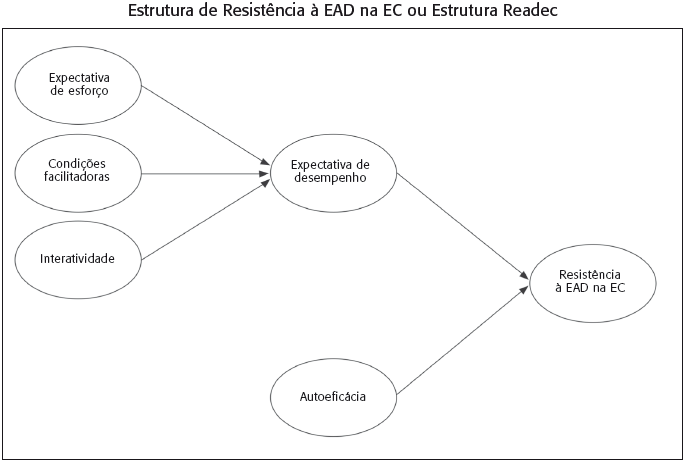
\includegraphics[width=1\textwidth]{Readec.png}
            \end{center}
            \caption{Estrutura de resistência à EAD na EC ou Estrutura Readec(Albertim, Brauer, 2012\cite{Albertin_Brauer_2012})}
            \label{fig:Readec}
\end{figure}

Apesar das dificuldades apresentadas, o modelo de Educação a distância continua apresentando bons resultados nos quesitos de escalabilidade, replicabilidade e flexibilidade para os alunos, tornando-o muito desejável para o âmbito das Universidades Corporativas, além de apresentar a possibilidade a empresas de menor porte, sem os recursos para manter tais estruturas, de contrata-los como serviços com maior facilidade, gerando a possibilidade de mitigar parcialmente os altos custos de implementação iniciais das Universidades Corporativas. 

Em seu artigo "As comunidades virtuais como instrumento de educação corporativa: estudo de caso no Tribunal de Contas da União", Mathias e Santos (2014, \cite{Mathias_Santos_2014}) levantam a visão da educação corporativa contínua, não limitada a treinamentos  pontuais, e apresentam as comunidades virtuais  como ferramentas para criar um ambiente de aprendizado contínuo, assim como uma cultura de aprendizado. Os autores apontam a origem do modelo educacional tradicional na sociedade industrial moderna, e seu objetivo de capacitação pontual, posto que as capacidades requeridas neste ambiente possuíam pouca variabilidade ao longo do tempo. Os autores contrastam esta realidade com a sociedade informacional em que estamos inseridos, na qual as demandas de adaptabilidade e aprendizado são elementos centrais da prática profissional em todos os níveis, assim como de todas as áreas de negócios. Consequentemente, os autores apontam a necessidade de adequar as estruturas de aprendizagem para esta nova realidade, voltando o foco dos setores de capacitação profissional da eficiência operacional para a compreensão e respeito ás estratégias organizacionais da empresa, como indica a figura 3.4.

De acordo com os autores, as comunidades virtuais, possibilitadas por Tecnologias Digitais de Informação, Comunicação e Expressão (TDICE) tem sua implantação em ambientes de educação corporativa dificultada principalmente pela resistência de profissionais "imigrantes digitais", ou seja, nascidos ou formados antes da explosão da computação e da Internet, que ainda apresentam resistência ao seu uso intensivo. Os autores indicam que muitos profissionais ainda enxergam ambientes  virtuais de comunicação como espaços "para que os indivíduos possam fazer amigos, trocar fotos, conversar, enfim, interagir sobre aspectos que não pertencem ao ambiente profissional ou educacional." Os autores apresentam como principais vantagens do uso de comunidades virtuais no âmbito da educação corporativa a facilidade de aprendizagem continuada; a possibilidade de discussão  e, consequentemente, inovação sobre os temas abordados; a criação de um repositório comum de conhecimento, facilitando tanto a capacitação de novos funcionários, quanto a aprendizagem de funcionários existentes sobre áreas outras que a sua, facilitando a colaboração entre diferentes áreas de uma empresa; e a disseminação de conhecimento relativo a mudanças. Os autores apontam o uso das TDICEs como recursos de aprendizagem adequados a uma abordagem sociointeracionista da educação, fundamentada pelos estudos desenvolvidos por Vygotsky, Wallon, e Piaget, entre outros, que apontam que o indivíduo aprende pela interação com o outro. 








\begin{figure}
            \begin{center}
                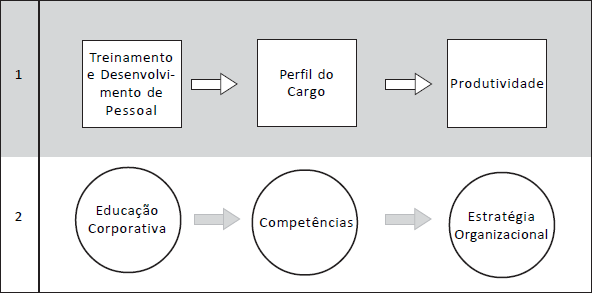
\includegraphics[width=1\textwidth]{Treinamento_v_educacao.png}
            \end{center}
            \caption{Treinamento e educacao(Mathias e Santos, 2014\cite{Mathias_Santos_2014})}
            \label{fig:Treinamento_v_Educacao}
\end{figure}

